\chapter{System Design- The Box}

The Box is a stand alone, modular incubator that will be used to let certain SE3D experiments culture over an extended period of time. It will provide a custom lighting environment that allows consistent lighting conditions for the camera to effectively document the experiments. The box also will have temperature control capabilities to adjust temperature levels for each of the relevant SE3D experiments. The box will support nine petri dishes at one time.

\begin{figure}[H]
\caption{\label{figure:box} Initial Incubator Prototype}
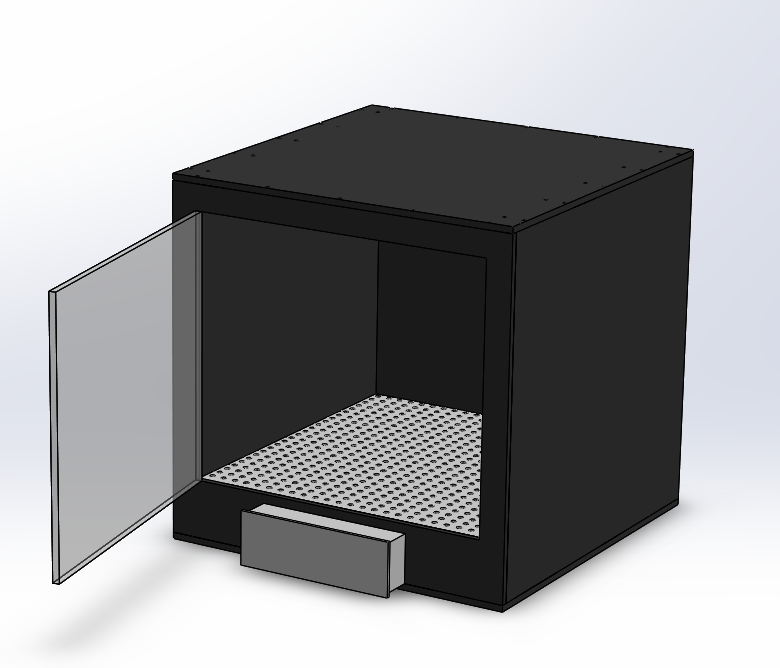
\includegraphics[scale=0.5]{box}
\end{figure}

Figure \ref{figure:box} shows a initial drawing of the plans for the physical incubating box. At the top of the box, there will be a touch screen that allows users to interact with the controls of The Box.



\section{Architectural Design}
\section{Conceptual Model}

The user interface for The Box consists of screens in which the user can configure the box’s settings for the current experiment, begin and end experiments, and download images that are collected during the experiment. The user interface shall perform the following: 

\begin{enumerate}
	\item	Run off of a microcomputer
	\item	Allow users to choose custom light, temperature, and image capture settings
	\item	Allow users to load a previously saved environment 
	\item	Organize all images from a single experiment into a folder per petri dish so that they each can be exported to USB 

\end{enumerate}
\begin{figure}[H]
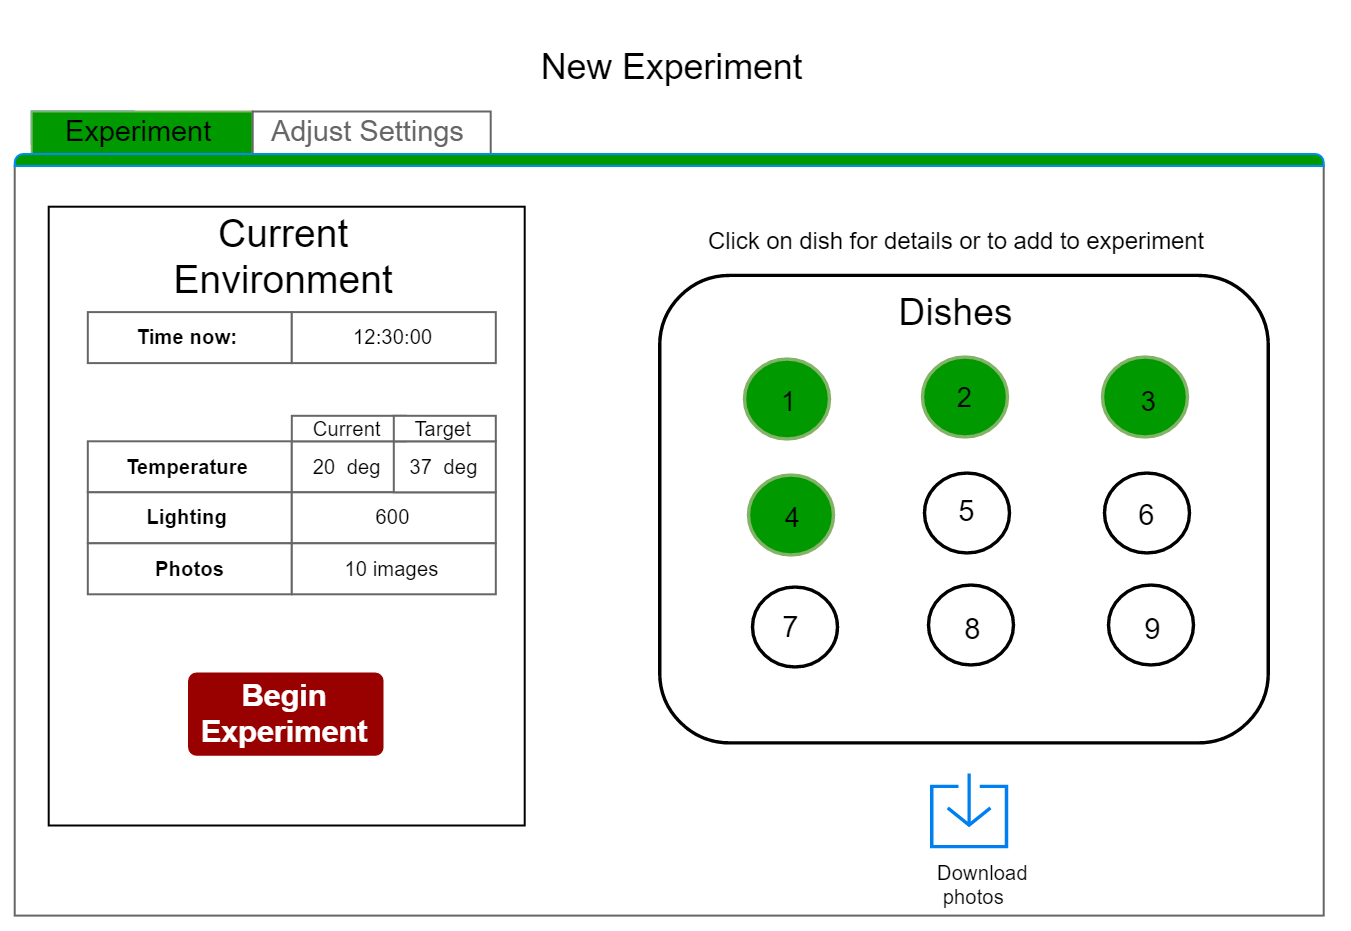
\includegraphics[scale=0.5]{ui-home-screen}
\caption{\label{figure:ui-home} Mock up of home screen}
\end{figure}

\begin{figure}[H]
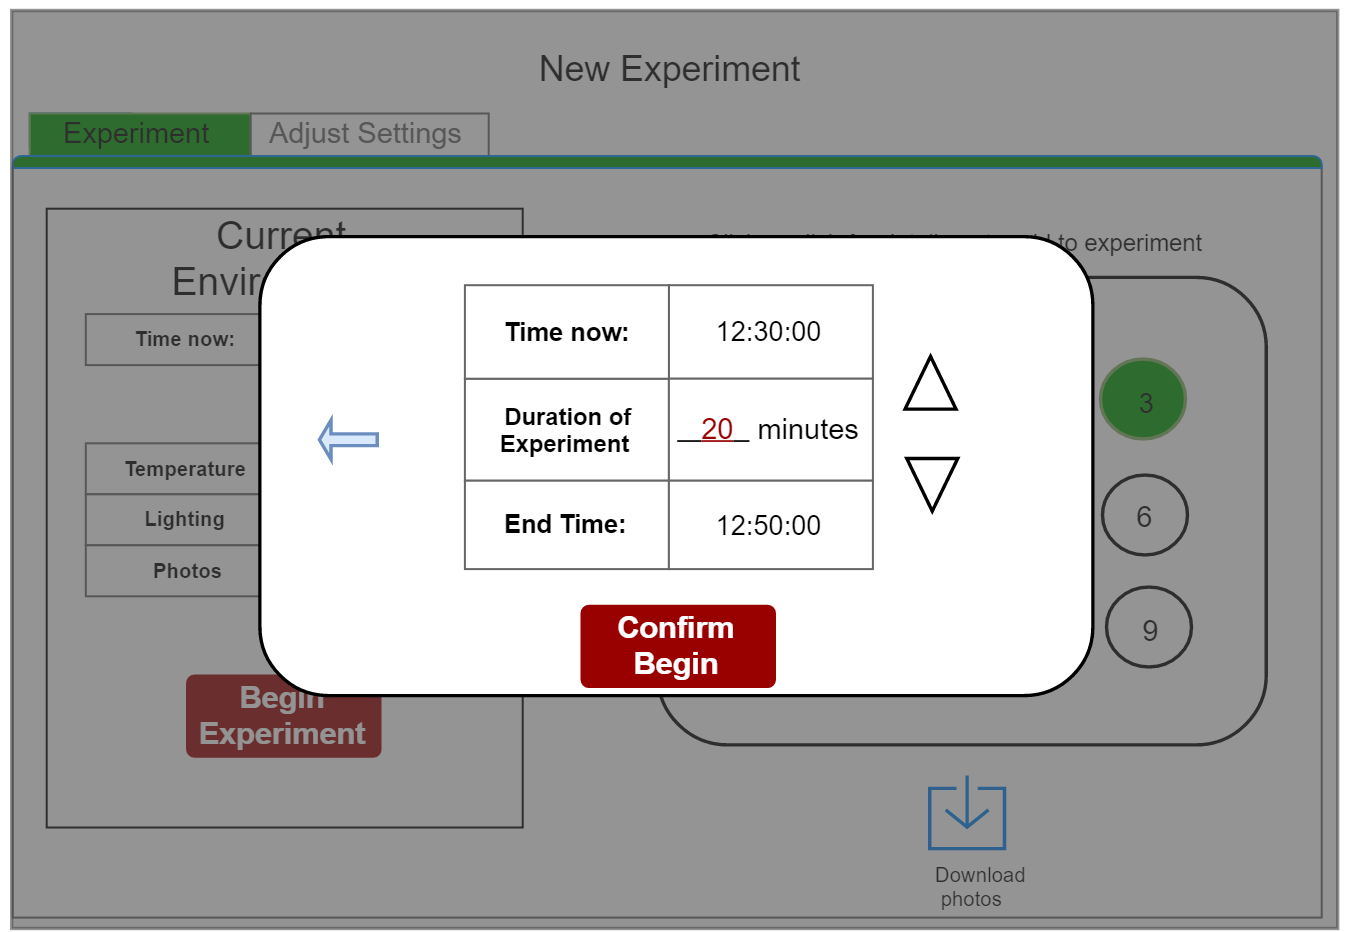
\includegraphics[scale=0.5]{ui-begin}
\caption{\label{figure:ui-begin} Mock up confirming experiment begin }
\end{figure}

\begin{figure}[H]
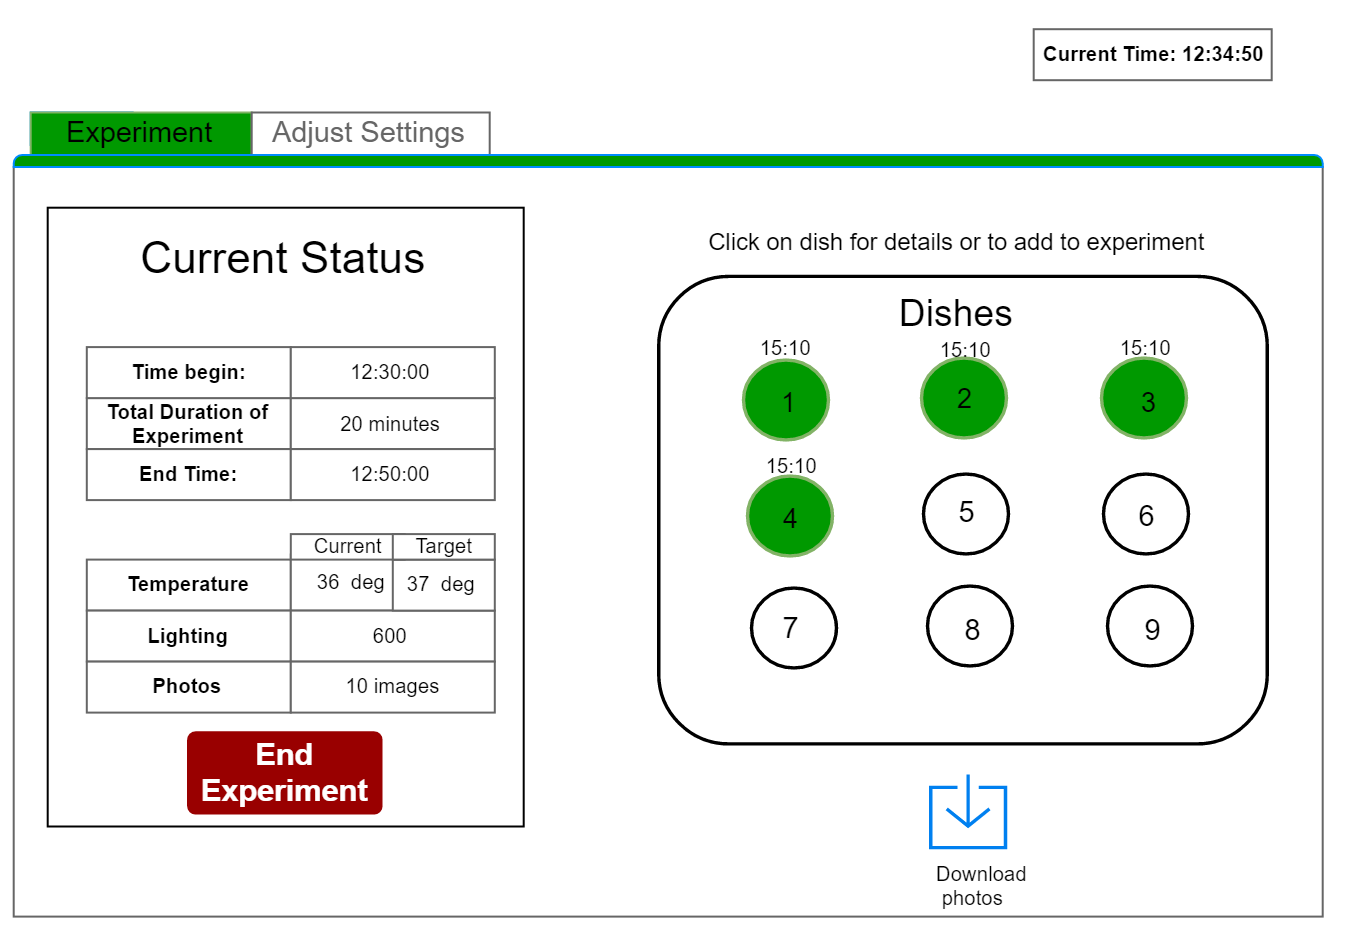
\includegraphics[scale=0.5]{ui-status-1}
\caption{\label{figure:ui-status} Mock up of status screen during an experiment}
\end{figure}

\begin{figure}[H]
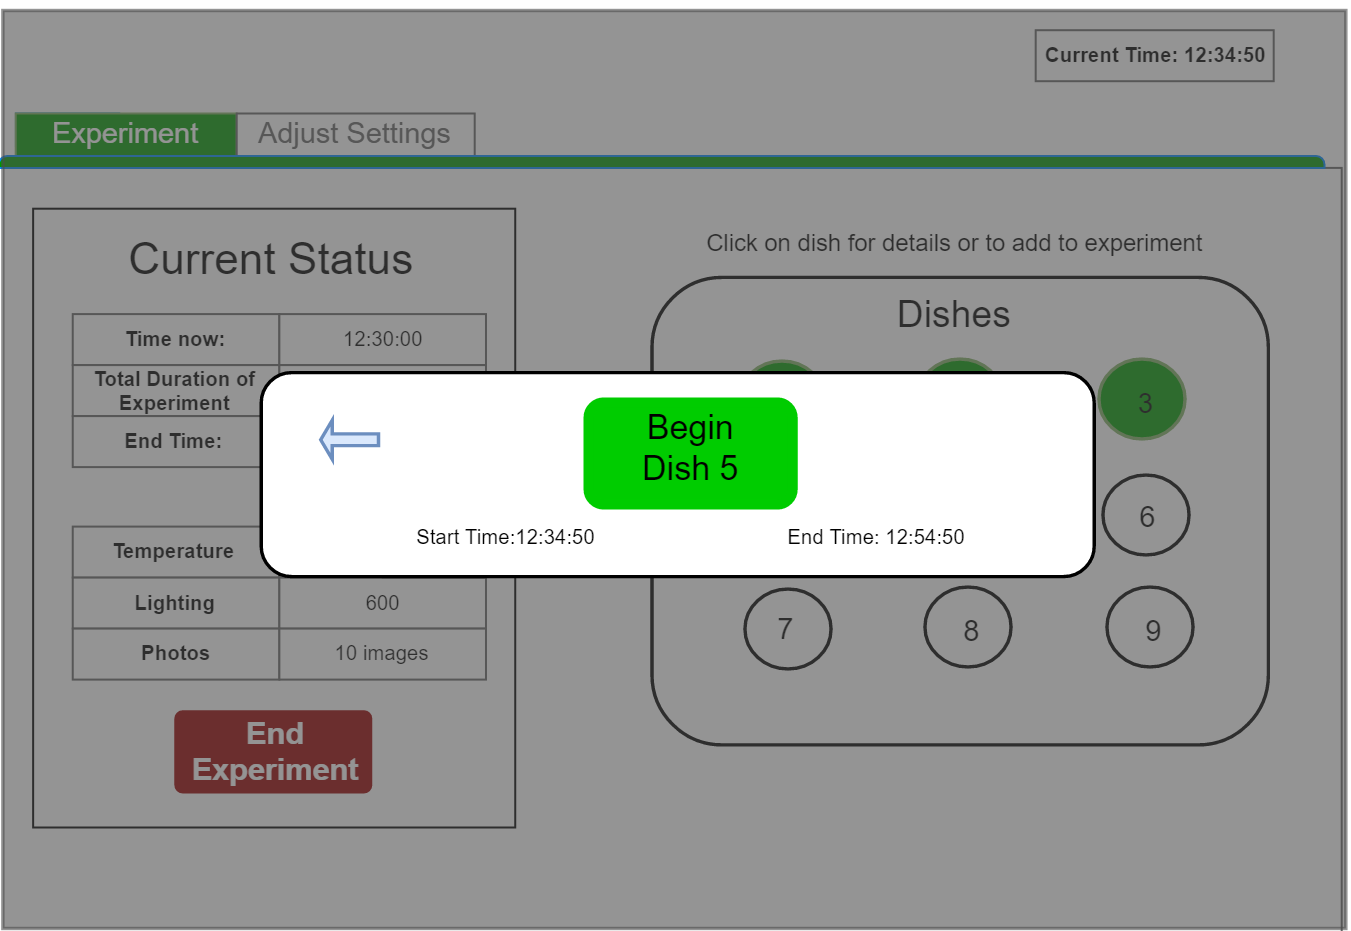
\includegraphics[scale=0.5]{ui-add-dish}
\caption{\label{figure:ui-add} Mock up of how a dish is added in the middle of an experiment}
\end{figure}

\begin{figure}[H]
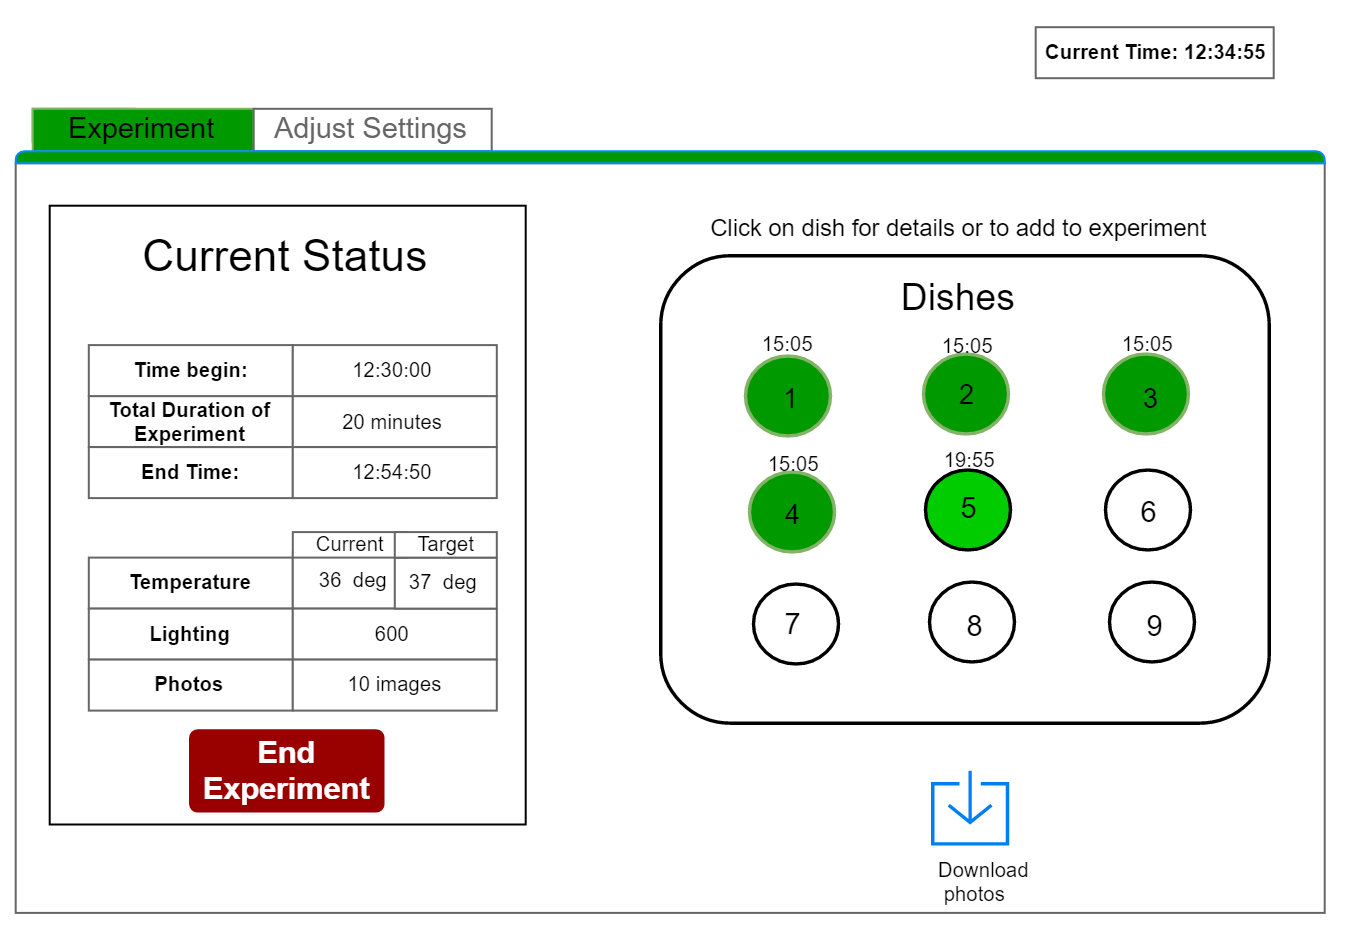
\includegraphics[scale=0.5]{ui-after-add}
\caption{\label{figure:ui-after-add} Mock up of how current status screen reflects addition of a dish}
\end{figure}

\begin{figure}[H]
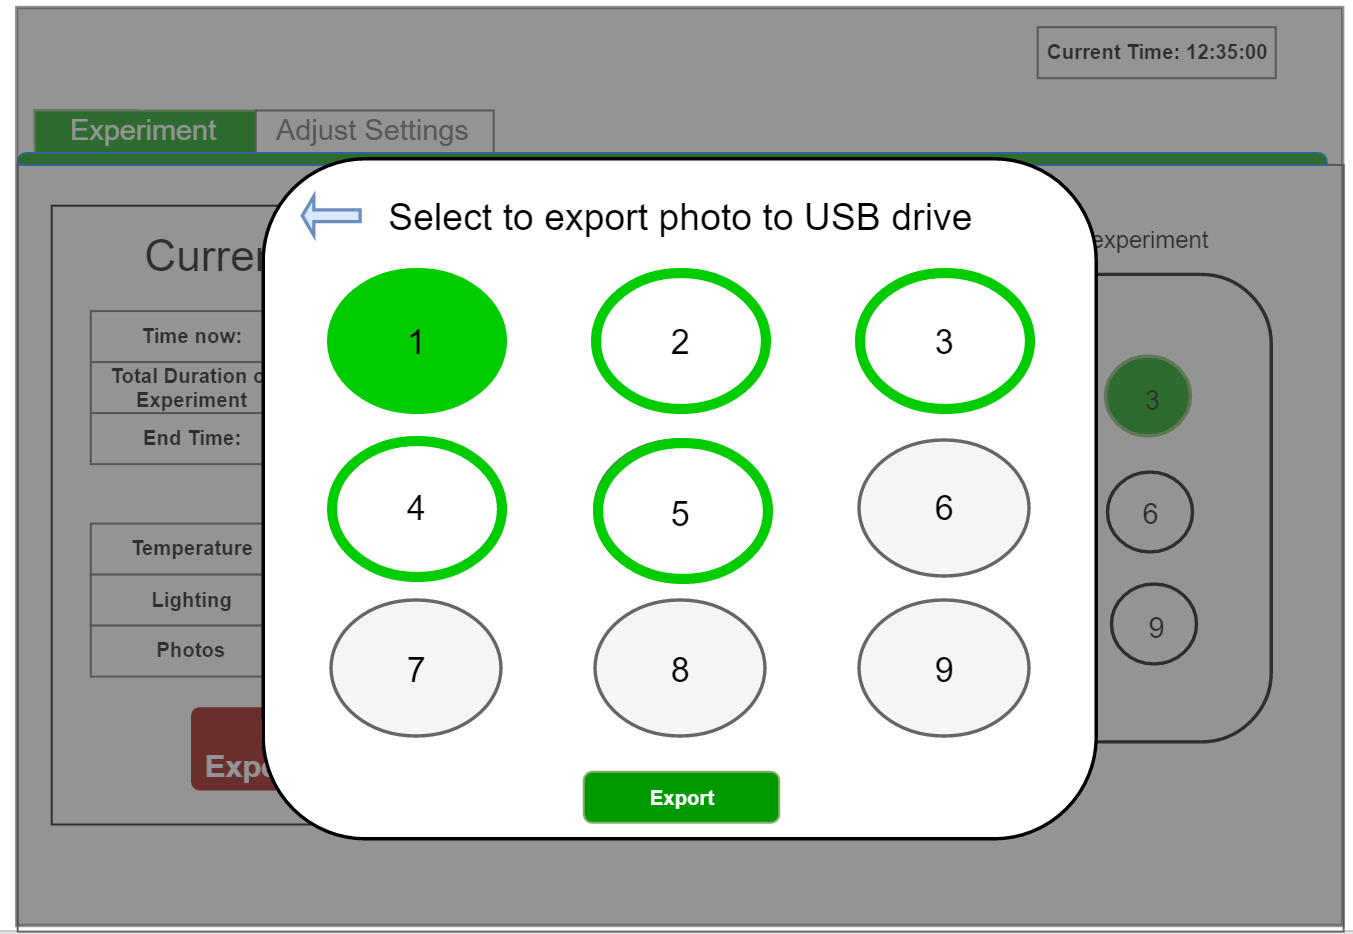
\includegraphics[scale=0.5]{ui-export}
\caption{\label{figure:ui-export} Mock up of export images to a USB drive}
\end{figure}

\begin{figure}[H]
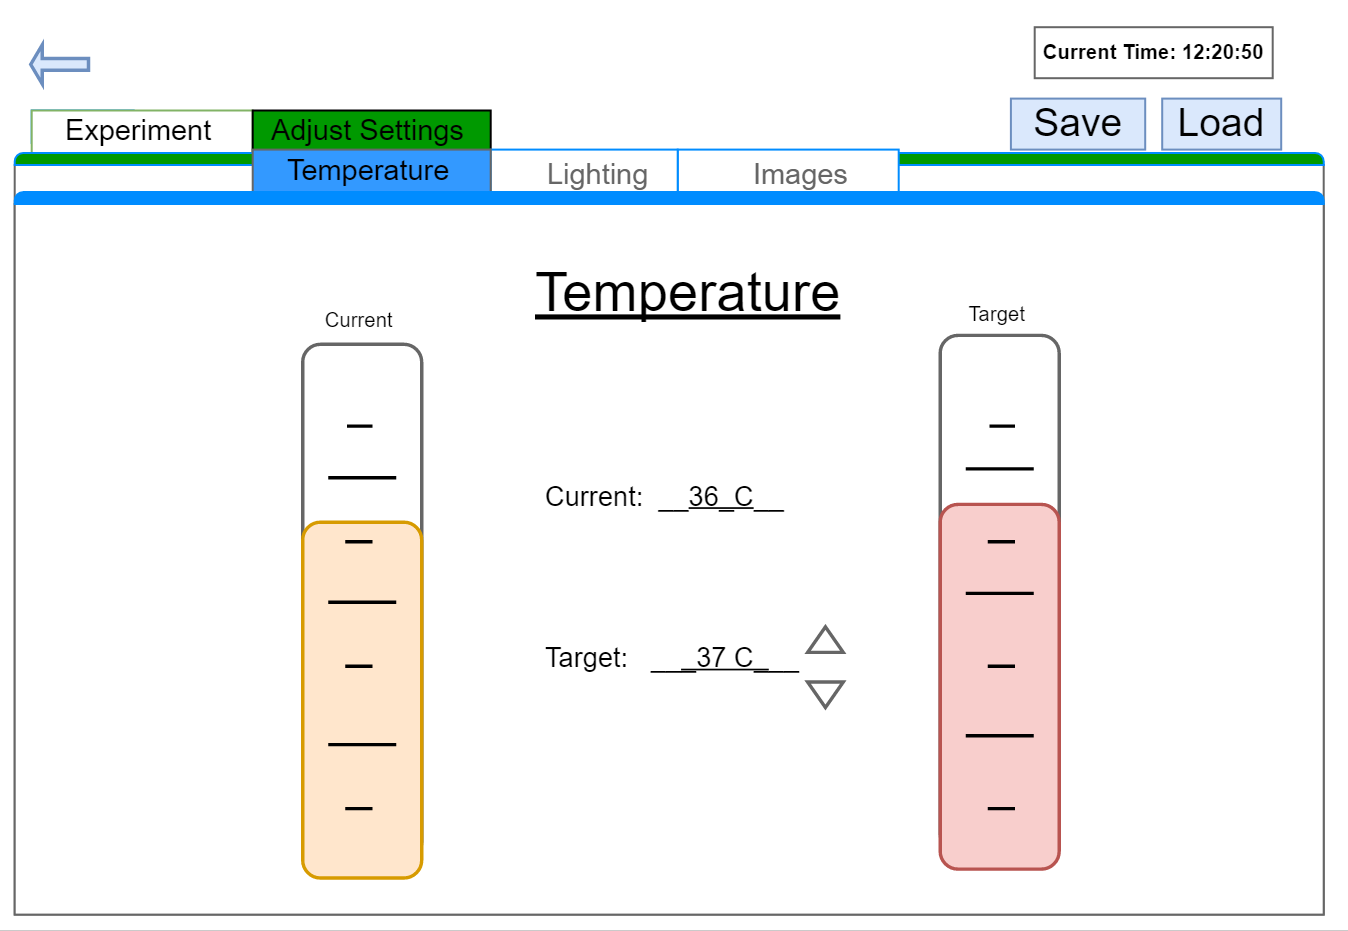
\includegraphics[scale=0.5]{ui-temp}
\caption{\label{figure:ui-temp} Mock up of temperature setting}

\end{figure}

\begin{figure}[H]
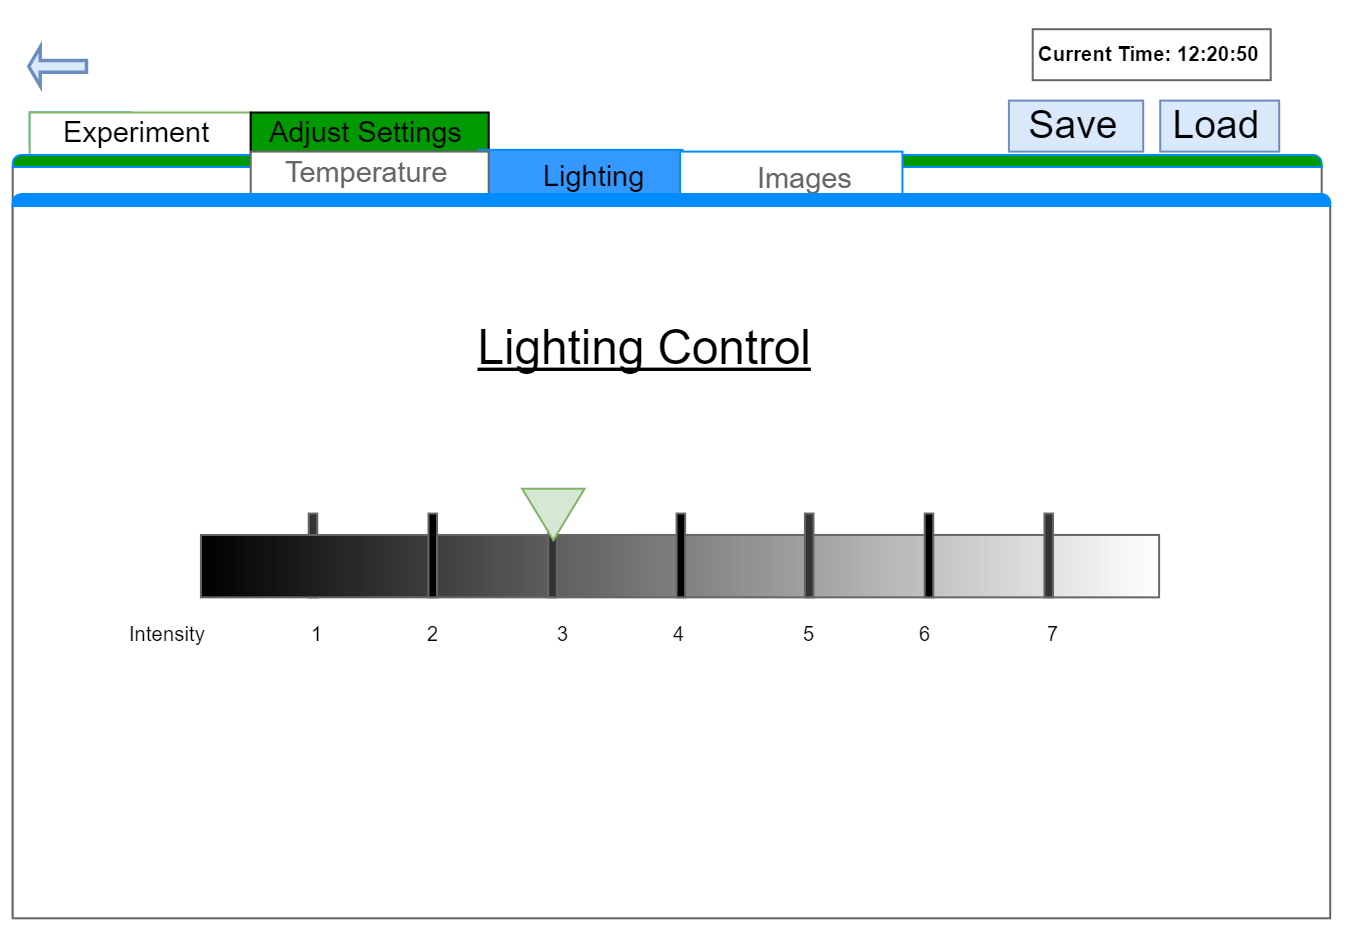
\includegraphics[scale=0.5]{ui-light}
\caption{\label{figure:ui-light} Mock up of light intensity setting}
\end{figure}

\begin{figure}[H]
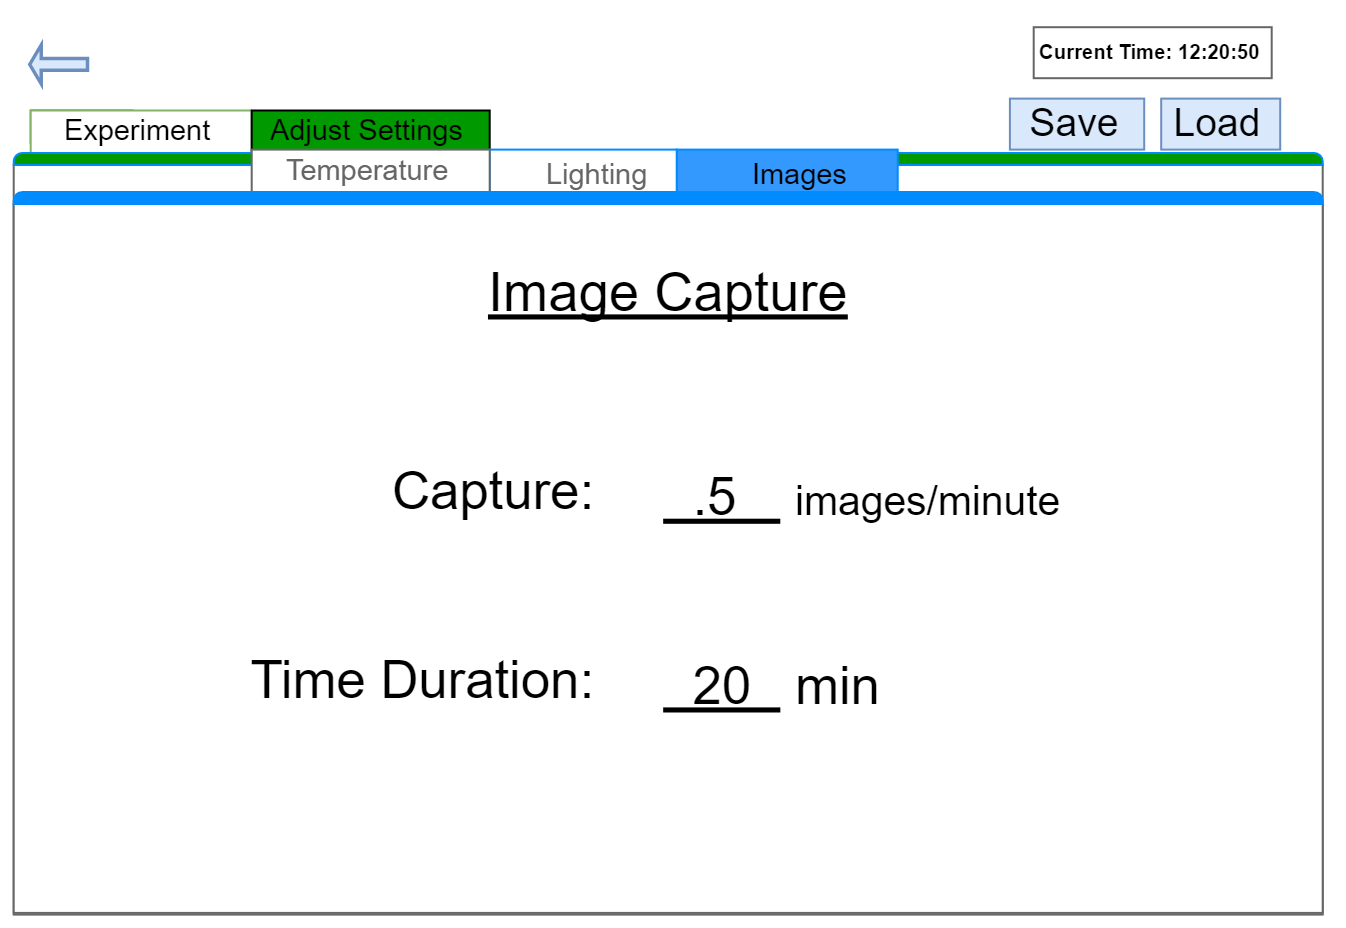
\includegraphics[scale=0.5]{ui-image}
\caption{\label{figure:ui-image} Mock up of image capture setting}
\end{figure}

\section{Design Rationale}
\subsection{Justification of User Experience}
\subsection{Justification of Technologies Used}
\section{Technologies Used}